\chapter{Digitální rádio a metody komprese audiosignálu}
\label{chap.digitalRadio}

\epigraph{\textit{\hfill Video killed the radio star.}}{The Buggles, \textit{název písně}}

Přestože smrt rádia prorokovali \uv{The Buggles} v historicky prvním videoklipu vysílaném hudební televizí MTV (\textit{Music Television}), analogové rádio je tu s námi dodnes a v následujících letech pravděpodobně bude i nadále. Zdá se že minimálně do roku 2025, dokdy v České Republice platí licence na pásma, ve kterých je klasické FM rádio provozováno. Nicméně digitalizace je všudypřítomný trend a podobně jako se v průběhu poslední dekády přecházelo na digitální vysílání televize DVB-T (\textit{Digital Video Broadcasting – Terrestrial}), čeká nás modernizace i ve vysílání rozhlasových služeb. 

\section{Standardy digitálního rozhlasového vysílání}

V současné době existují dva velké paralelně existující standardy. DAB (\textit{Digital Audio Broadcasting}), ke kterému se po úspěchu v severských zemích upínají i tuzemští poskytovatelé rozhlasových služeb, a DRM (\textit{Digital Radio Mondiale}), momentálně zažívající \uv{boom} v Indii a dalších zemích, kde je rádio provozováno v pásmu středně dlouhých vln. Vedle nich existují i další systémy, jako například Japonský ISDB (\textit{Integrated Services Digital Broadcasting}) standard pro vysílání televize a rádia, nahrazující tamější analogový NTSC-J (\textit{National Television System Committee - Japan}), či IBOC (\textit{In-band on-channel}) užívaný v Americe pod obchodním názvem HD Radio, který vysílá analogový a digitální signál simultánně. Tyto druhy vysílání se ovšem nevztahují k evropské půdě a tudíž se práce v následujících dvou podkapitolách zabývá pouze systémy DAB/DAB+ a DRM(+).

\subsection{Digital Audio Broadcasting}

Standard \textit{EUREKA 147 Digital Audio Broadcasting} (zkráceně DAB) popsaný v normě ETSI EN 300 401\cite{etsi:dab} je normou vyvíjenou již od osmdesátých let Evropským ústavem pro telekomunikační normy ETSI (\textit{European Telecommunications Standards Institute}) společně s Mezinárodní telekomunikační unií ITU (\textit{International Telecommunication Union}). Jedná se o moderní a univerzální multimediální rozhlasový systém, jehož cílem je nahradit současné FM vysílání. Oproti tomu se pyšní například odolností vůči aditivnímu šumu, kvalitou zvuku srovnatelnou se záznamem na CD, energetickou úsporností a možností využití ve více pásmech. Balík několika rozhlasových stanic společně s doprovodnými datovými službami multiplexuje do jednoho datového toku, který je poté vysílán modulací OFDM (\textit{Orthogonal frequency-division multiplexing}), jejíž hlavní předností je odolnost vůči chybám způsobeným vícecestným šířením a možnost využití jedno-frekvenční sítě.

%\subsection{Vysílací módy}

Starší verze systému DAB \cite{etsi:dab:old}, byla navržena pro přenos různými technologiemi v několika pásmech jak je ukázáno v tabulce \ref{table:dab}. Definovány byly 4 vysílací módy, které umožňovaly vysílání až do frekvencí kolem 3 GHz. Ve verzi 2.2.1 doporučení ETSI EN 300 401 \cite{etsi:dab} z ledna 2017 se už s módy II - IV nadále nepočítá a DAB+ tak zůstává ryze terestrickou platformou.

\begin{table}[ht]
\centering
\begin{tabular}{|c|c|c|c|c|}
\hline
\textit{\textbf{}} & \textbf{Mód I} & \textbf{Mód II} & \textbf{Mód III} & \textbf{Mód IV} \\ \hline
Použití & \begin{tabular}[c]{@{}c@{}}Pozemní \\ VHF\\  168 - 240 MHz\end{tabular} & \begin{tabular}[c]{@{}c@{}}Pozemní \\ L pásmo\\  1452 - 1492 MHz\end{tabular} & \begin{tabular}[c]{@{}c@{}}Satelitní \\ L pásmo\\ až do 3 GHz\end{tabular} & \begin{tabular}[c]{@{}c@{}}Městská \\ zástavba\\  L pásmo\end{tabular} \\ \hline
\begin{tabular}[c]{@{}c@{}}Počet nosných vln\\ frekvencí\end{tabular} & 1536 & 384 & 192 & 768 \\ \hline
\begin{tabular}[c]{@{}c@{}}Odstup nosných vln\\ {[}kHz{]}\end{tabular} & 1 & 4 & 8 & 2 \\ \hline
\begin{tabular}[c]{@{}c@{}}Trvání intervalu \\ {[}$\mu$s{]}\end{tabular} & 1246 & 311,5 & 155,75 & 623 \\ \hline
\begin{tabular}[c]{@{}c@{}}Délka ochranného\\ intervalu\end{tabular} & 246,0 & 61,5 & 30,75 & 123 \\ \hline
\end{tabular}
\caption{Provozní módy DAB/DAB+ \cite{etsi:dab}}
\label{table:dab}
\end{table}

%\subsection{Principy}

Norma \cite{etsi:dab} definuje pouze vznik signálu na vysílací straně. Řešení na přijímací straně je ponecháno na výrobci koncových zařízení. Na obrázku \ref{pic:dab} je ukázáno jak je sestavení DAB signálu řešeno.

\begin{figure}[h]
    \centering
    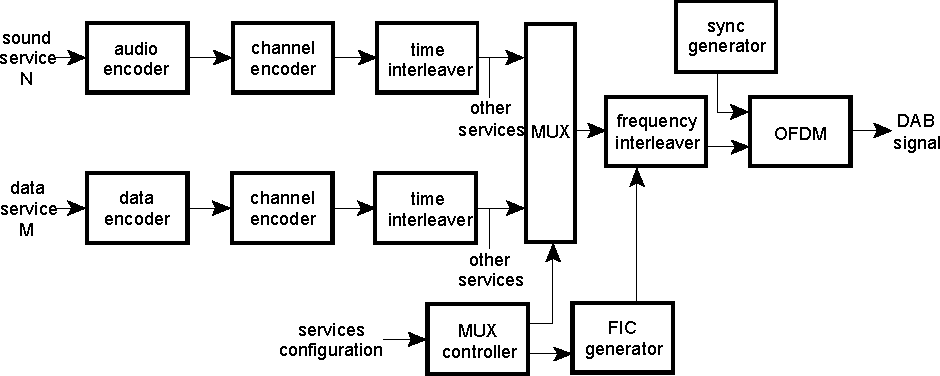
\includegraphics[width=.9\textwidth]{pic/dab.pdf}
    \caption{Blokové schéma sestavení DAB/DAB+ signálu.\cite{etsi:dab}}
    \label{pic:dab}
\end{figure}

Z hlediska zdrojového kódování využívá původní DAB kodek MPEG-1 Audio Layer II (více o kodecích v podkapitole \ref{subchap:codecs}). Je možno použít dva vzorkovací kmitočty: 24 kHz a 48 kHz. Od těch se odvíjí možné bitové rychlosti zdrojového kódování vypsané v tabulkách \ref{table:dabbitrates1} a \ref{table:dabbitrates2}. Výstupem kodéru jsou logické rámce (\textit{Logical Frames}) trvající 48 ms respektive 24 ms pro vyšší vzorkovací rychlost.
V novější verzi DAB+ metodu MPEG Layer II doplnil modernější  kódovací postup HE-AAC v2. Tok nového kodéru je opatřen Reed-Solomonovým ochranným kódem a je vkládán do superrámců (\textit{Super Frames}), dlouhých 120 ms, které jsou rozděleny do pěti logických rámců DAB. Počet vzorkovacích kmitočtů vyrostl na čtyři. Konkrétně: 16, 24, 32, 48 kHz a možné bitové rychlosti jsou násobky osmi od 8 kb/s až do 192 kb/s.

\begin{table}[h]
\centering
\begin{tabular}{|c|c|c|c|c|c|c|c|c|}
\hline
48 kHz jednokanálový mód (kb/s) & 56 & 64 & 80 & 96 & 112 & 128 & 160 & 192 \\ \hline
48 kHz ostatní módy (kb/s) & 112 & 128 & 160 & 192 & 224 & 256 & 320 & 384 \\ \hline
\end{tabular}
\caption{Dostupné bitové rychlosti při použití MPEG Layer II a vzorkovací rychlosti 48 kHz \cite{etsi:mp2}}
\label{table:dabbitrates1}
\end{table}

\begin{table}[h]
\centering
\begin{tabular}{|c|c|c|c|c|c|c|c|c|c|c|c|c|c|c|}
\hline
24 kHz (kb/s) & 8 & 16 & 24 & 32 & 40 & 48 & 56 & 64 & 80 & 96 & 112 & 128 & 144 & 160 \\ \hline
\end{tabular}
\caption{Dostupné bitové rychlosti při použití MPEG Layer II a vzorkovací rychlosti 24 kHz \cite{etsi:mp2}}
\label{table:dabbitrates2}
\end{table}


Po odstranění irelevantních a nadbytečných dat zdrojovým kodérem, přichází na řadu přidání pečlivě řízené redundantní složky pomocí konvolučního kodéru, který je následován časovým prokladačem. Ten determinovaným způsobem přeskládá tok dat tak, že při zpětném složení se případná shluková chyba, vzniklá při přenosu kanálem, \uv{rozmělní} a může být opravena konvolučním kódem. Maximální možné přenosové rychlosti multiplexu DAB v závislosti na stupni ochrany jsou v tabulce \ref{table:dabcoderates}.

\begin{table}[h]
\centering
\begin{tabular}{|c|c|c|}
\hline
Stupeň ochrany & Kódový poměr & Kapacita multiplexu (kb/s) \\ \hline
1-A & 1/4 & 576 \\ \hline
2-A & 3/8 & 864 \\ \hline
3-A & 1/2 & 1152 \\ \hline
4-A & 3/4 & 1728 \\ \hline
\end{tabular}
\caption{Přehled dostupných přenosových rychlostí v DAB/DAB+ pro dostupné stupně ochrany a kódové poměry}
\label{table:dabcoderates}
\end{table}

Počet programů v multiplexu DABu je flexibilní, zrovna tak jako nastavení kvality jednotlivých zvukových služeb a jejich doprovodných informací.

Ortogonálně frekvenčně dělený multiplex, neboli OFDM je modulace využívající velkého množství nosných vln. Dostupná šířka pásma je rozdělena do ortogonálních subkanálů. Ty jsou od sebe vzdáleny $\Delta f = \frac{1}{T}$, kde $T$ je doba trvání jednoho symbolu. Signál omezený v čase si lze představit jako signál trvající nekonečně dlouho vynásobený obdélníkovým pulzem. Takovému signálu ve frekvenčním spektru odpovídá výkonová hustota popsaná funkcí $\frac{\sin{x}}{x}$. Průchody nulou jednotlivých nosných vln jsou umístěny přesně na sebe, díky čemuž jsou postranní laloky potlačeny, jak naznačuje obrázek \ref{pic:ofdm}.

\begin{figure}[h]
    \centering
    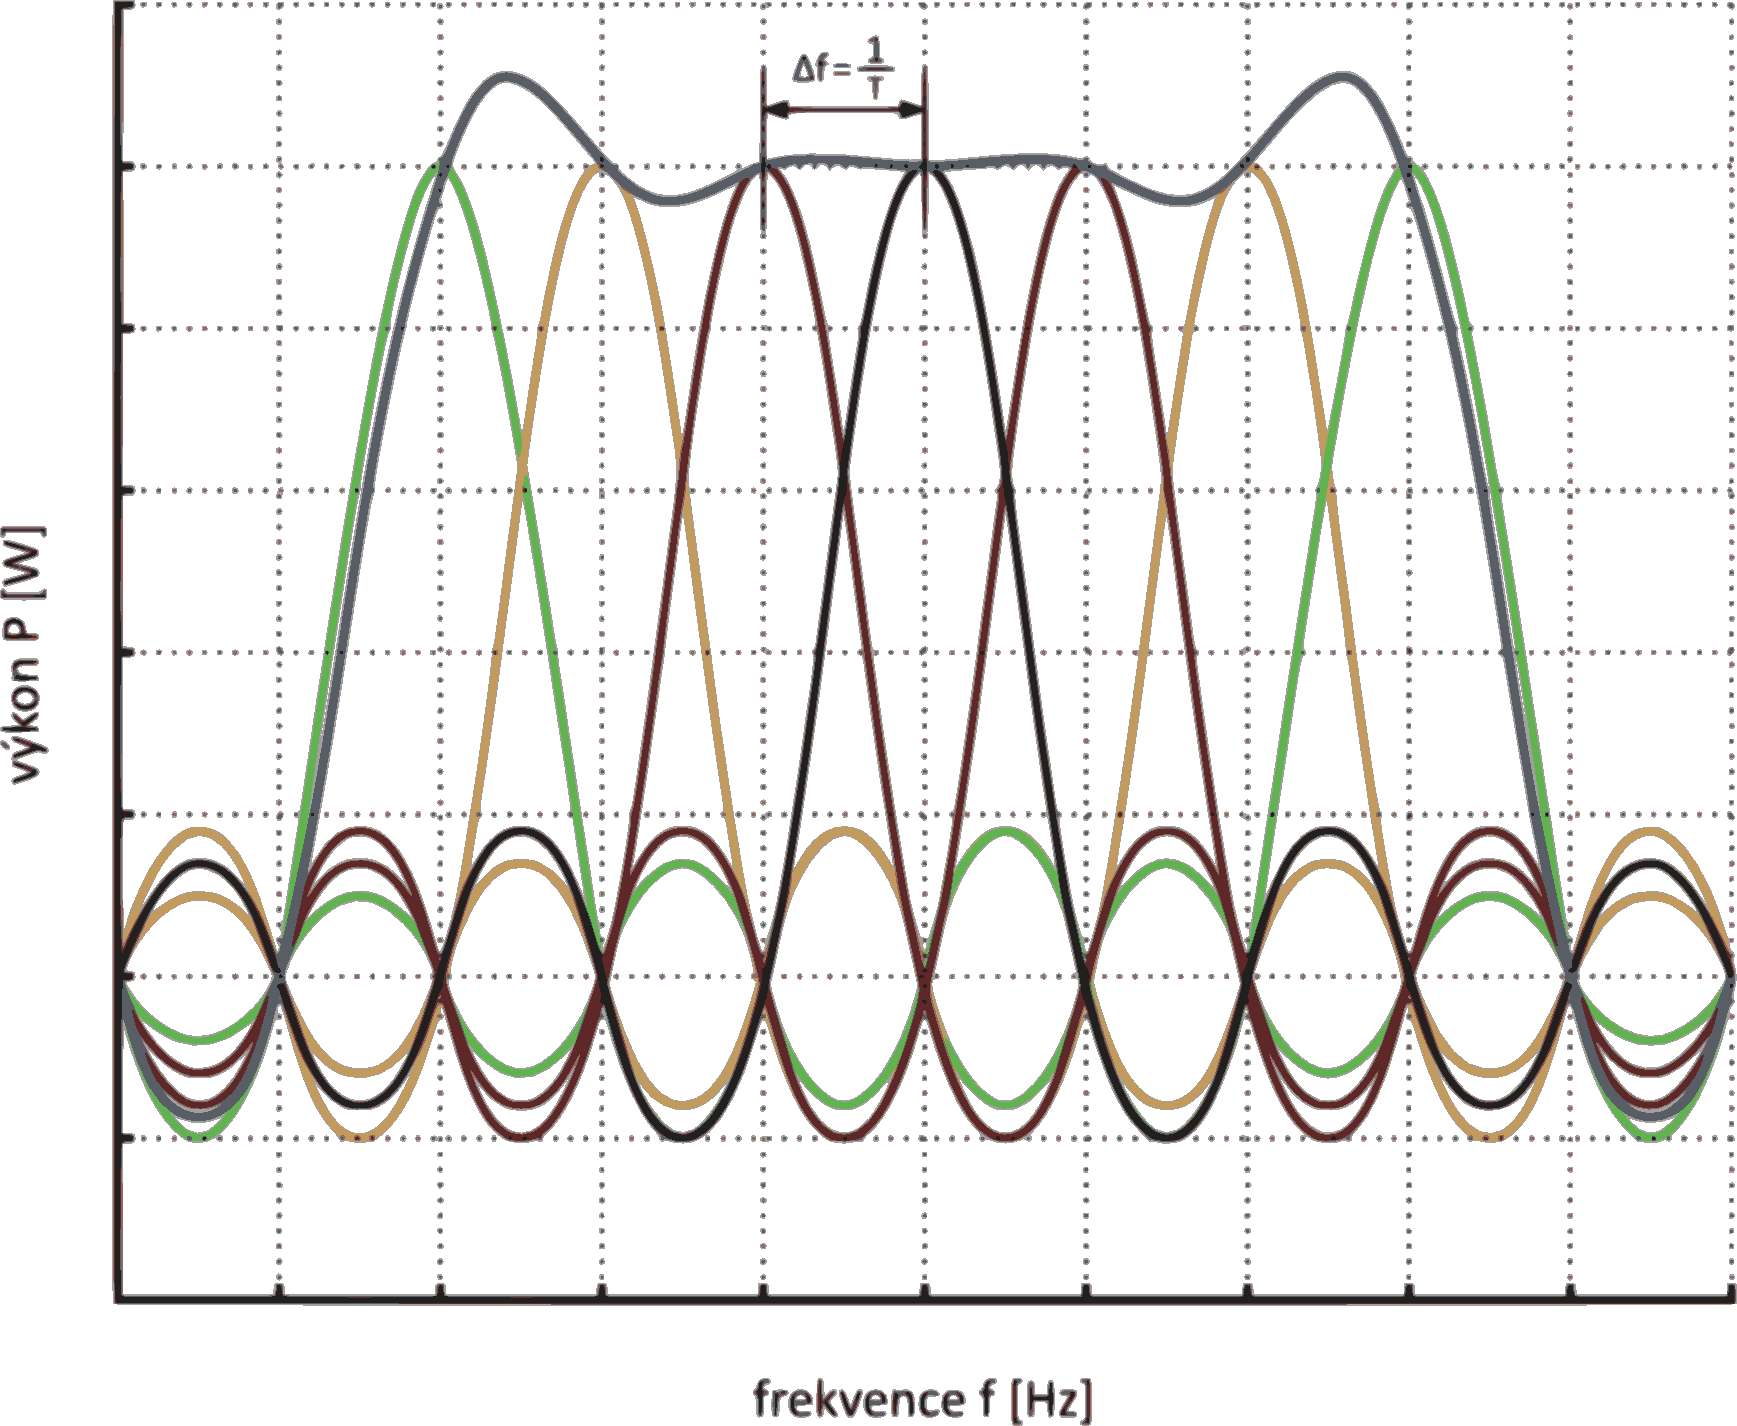
\includegraphics[width = .5\textwidth]{pic/ofdm2.pdf}
    \caption{Naznačení principu rozmístění nosných kmitočtů v systému OFDM \cite{web:ofdm}}
    \label{pic:ofdm}
\end{figure}


K čemu velké množství nosných frekvencí? Zjednodušeně řečeno, čím více nosných vln, tím delší symbolový čas $T$. Odražený signál, který do přijímače dorazí s časovým zpožděním může způsobit chybnou detekci symbolu. Dobře se to dá představit na analogové televizi, kde zpožděný signál způsobil chybu známou jako \uv{duch}. V digitálním světě sice \uv{duchové} neexistují, zato vznikne překryv symbolu zpožděného signálu se symbolem následujícího rámce, tedy jev známý jako mezisymbolová interference ISI (\textit{Inter Symbol Interference}). Prodloužení symbolového času způsobí to, že mírně zpožděný signál dorazí stále \uv{včas} a nedojde k znehodnocení přijatého symbolu. I přesto ve zlomku vysílacího času vzniká překryv dvou symbolů a proto je do vysílání vkládán ochranný interval GI (\textit{Guard Interval}), neboli čas, kdy je vysílání pozastaveno. Tím na jednu stranu klesá efektivita přenosu, nicméně signál je díky tomu značně odolnější vůči odrazům. Zároveň to umožňuje konstruovat sítě s vysílači na téže frekvenci, čímž dochází k značné úspoře spektra.    

Jednotlivé nosné vlny jsou v systému DAB modulovány čtyř stavovým fázovým klíčováním s pamětí neboli DQPSK (Differential Quadrature Phase-Shift Keying).

\subsection{Digital Radio Mondiale (+)}


Na rozdíl od systému DAB, který postupně nahrazuje FM vysílání pouze v pásmu velmi krátkých vln, si DRM brousí zuby i na stanice vysílané amplitudovou modulací ve středních a dlouhých vlnách. ETSI ho definuje normou \textit{ETSI ES 201 980} \cite{etsi:drm}, a k dnešnímu dni existují jeho dvě verze: DRM30 a DRM+. Novější verze standard doplnila o módy pro použití v pásmu VKV a také o modernější druhy zdrojového kódování.

%\subsection{Principy}

Blokové schéma vysílače DRM je znázorněno na obrázku \ref{pic:drm}. V Multiplexu systému DRM je ve srovnání s digitálním rádiem DAB podstatně menší počet rozhlasových stanic. Typicky jedna, maximálně však čtyři (včetně doplňkových dat). To může být výhodou pro poskytovatele obsahu. Odpadá jim tak problematika složitého domlouvání se s konkurencí a tím je mimo jiné zajištěna větší nezávislost. 

\begin{figure}[h]
    \centering
    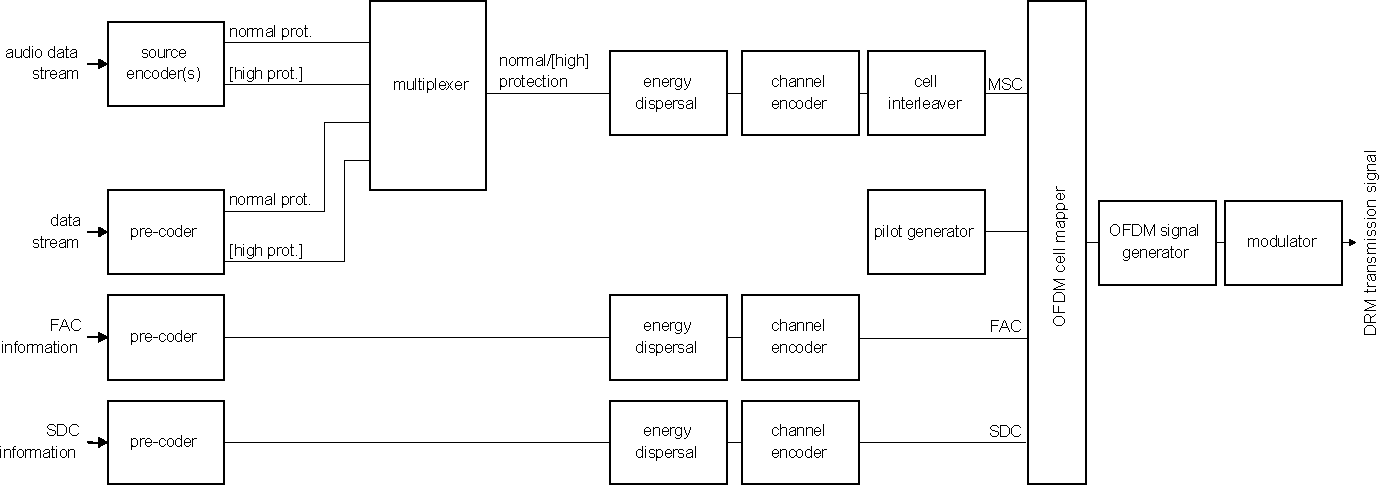
\includegraphics[width=1\textwidth]{pic/drm.pdf}
    \caption{Blokové schéma DRM systému \cite{etsi:drm}}
    \label{pic:drm}
\end{figure}

Pro kanály umístěné ve spektru pod hranicí 30 MHz, nabízí DRM vzhledem k použité modulaci prostor pro datový tok od 8 kb/s po 72 kb/s. Pro kanály nad 30 MHz maximální bitová rychlost povyroste až na 186 kb/s. Nabídka systémů zdrojového kódování je následující:
\begin{itemize}
    \item MPEG-4 CELP, MPEG-4 XVHC - pro monofonní kódování mluveného slova
    \item MPEG-4 HE-AAC v2 - pro kódování hudebních stanic
    \item MPEG xHE-AAC - univerzální kodek pro řeč a hudbu
    \item MPEG Surround - pro kódování doplňkových stop při vícekanálovém přenosu
\end{itemize}

\smallskip

Výsledný datový tok se skládá ze třech kanálů:
\begin{itemize}
    \item MSC (\textit{Main Service Channel}) - kanál obsahující audio a datové služby
    \item FAC (\textit{Fast Acces Channel}) - informace určené k demodulování signálu 
    \item SDC (\textit{Service Description Channel}) - informace potřebné k dekódování MSC
\end{itemize}

Každý z bloků má svůj mírně specifický kanálový kodér. Scrambler zajišťuje pseudonáhodný charakter signálu, čímž vyrovnává výkon ve spektru. 

Poměr redundance přidané konvolučním kódováním je závislý na zvolené robustnosti. Z hlediska kanálu ve kterém lze DRM využívat definuje standard celkem pět typických prostředí (v tabulce \ref{table:drm_environment}) a k nim přiděluje možné kombinace nastavení modulace nosné vlny.


\begin{table}[h]
\centering
\begin{tabular}{|c|c|}
\hline
Mód & Typické podmínky prostředí \\ \hline
A & AWGN kanál, malé úniky \\ \hline
B & \begin{tabular}[c]{@{}c@{}}Časově a frekvenčně selektivní kanál s velkým\\ dopplerovským rozprostřením\end{tabular} \\ \hline
C & \begin{tabular}[c]{@{}c@{}}Jako B, ale s větší pravděpodobností \\ příjmu odraženého signálu\end{tabular} \\ \hline
D & \begin{tabular}[c]{@{}c@{}}Jako B, ale s extrémní pravděpodobností \\ příjmu odraženého signálu\end{tabular} \\ \hline
E & Časově a frekvenčně selektivní kanál \\ \hline
\end{tabular}\caption{Parametry OFDM symbolu.}
\label{table:drm_environment}
\end{table}

Konkrétní nastavení jsou vyjmenována v tabulce \ref{table:ofdm_drm}, kde časy v ní uvedené jsou vyjádřeny jako násobky elementární časové jednotky $T=83\sfrac{1}{3} ~\mathrm{\mu s}$. $T_u$ je čas trvání užitečné doby symbolu a $T_g$ je doba trvání ochranného intervalu.

\begin{table}[h]
\centering
\begin{tabular}{|c|c|c|c|c|c|}
\hline
Seznam Parametrů & \multicolumn{5}{l|}{Mód robustnosti} \\ \hline
 & A & B & C & D & E \\ \hline
$T_u$ [ms] & 288 $T$ & 256 $T$ & 176 $T$ & 112 $T$ & 27 $T$ \\ \hline
$T_g$ [ms] & 32 $T$ & 64 $T$ & 64 $T$ & 88 $T$ & 3 $T$ \\ \hline
$\sfrac{T_g}{T_u}$ & 1/9 & 1/4 & 4/11 & 11/14 & 1/9 \\ \hline
%$T_f$   [ms] & 400 & 400 & 400 & 400 & 100 \\ \hline
\end{tabular}
\caption{Parametry OFDM symbolu.}
\label{table:ofdm_drm}
\end{table}

OFDM má při terestrickém vysílání řadu výhod a i tento standard dělí kanál na velké množství navzájem se neovlivňujících nosných vln. K jejich modulaci je zde ale na výběr ze třech možností a to mezi čtyř, šestnácti a šedesáti čtyř stavovou kvadraturně amplitudovou modulací (4QAM,16QAM a 64QAM).

\section{Kodeky a profily používané v digitálním rozhlasovém vysílání}
\label{subchap:codecs}

V úvodu je zmíněno, že poznatky z psychoakustiky činí objektivní testování čím dál náročnější. Tato kapitola dává nahlédnout pod pokličku různých kódovacích metod jichž je v této práci užito. Výběr s jednou výjimkou, konkrétně kodeku Opus, ctí metody používané ve zdrojovém kódování v systémech digitálního rádia definovaných skupinou expertů pro pohyblivý obraz MPEG (\textit{Moving Picture Experts Group}).

\subsection{MPEG-1 Layer II}

Minulý rok tomu bylo již čtvrt století od momentu, kdy byl vydán standard ISO/IEC 111723 \cite{norm:mp2} zabývající se ztrátovou kompresí multimediálního obsahu. Jeho třetí část pojednávající o kódování audia definuje tři \uv{vrstvy}, jimiž se myslí úroveň integrace psychoakustických poznatků. Standard definuje částečnou dopřednou kompatibilitu jednotlivých vrstev, tedy schopnost alespoň částečně dekódovat tok dat z vyšší vrstvy dekodérem z vrstvy nižší. MPEG Audio Layer III komerčně známá pod označením \textit{mp3} se skrze kapesní přehrávače známe jako \uv{empétrojky} dostala do povědomí běžné veřejnosti, a i přes své stáří se těší úspěchu do dnešních dní.

V digitálním rádiu či televizním vysílání se ovšem používá její o něco méně komplexní verze MPEG Layer II. Na obrázku \ref{pic:mp2} je naznačen princip kódování.

\begin{figure}[h]
    \centering
    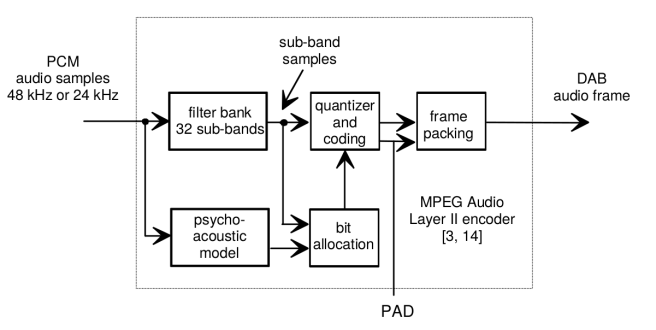
\includegraphics[width=.7\textwidth]{pic/mpeg2.png}
    \caption{Blokové schéma MPEG Layer II v systému DAB. \cite{web:mp2} }
    \label{pic:mp2}
\end{figure}

Vstupní pulzně kódovaný signál je rozdělen do dvou cest. V první z nich se nachází banka třiceti dvou filtrů, dělících signál do frekvenčních subpásem, která jsou poté kódována nezávisle. Blok zvaný psychoakustický model využívá principu zvaného spektrální sluchové maskování, neboli schopnosti lidského mozku nevnímat určité kmitočty, zní-li současně s nimi kmitočty jiné. Výstup tohoto bloku říká, jak hrubě kvantizovat (úrovňově rozdělit) jednotlivá subpásma.

Na takto upravené datové toky je poté použito Huffmanovo kódování, které častěji se vyskytujícím datovým slovům přiděluje kratší kódová slova. Tento princip je známý například z Morseovy abecedy. Konečnou fází je \uv{balení} dat do rámců a opatření hlavičkou obsahující data nezbytná pro dekodér.
 
\subsection{Advanced Audio Coding}

Standard AAC, přestavený jako součást specifikace MPEG-2, později doplněný o nové profily v MPEG-4 \cite{iso:aac} a MPEG-D je rodinou kodeků, která si klade za cíl poskytnout lepší poslechovou kvalitu, než \textit{mp3} při použití stejného bitového toku. Je postaven na modulárním přístupu. Podle potřeby lze využít různých rozšíření základního profilu a tím dosáhnout lepšího kódového zisku, efektivnějšího kódování řeči nebo například nižšího zpoždění. Na obrázku \ref{pic:aac} je naznačeno jakým způsobem jsou vrstveny profily používané v digitálním rádiu, popsané v následujících podkapitolách.

\begin{figure}[h]
    \centering
    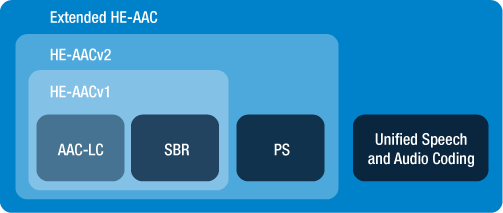
\includegraphics[width=.5\textwidth]{pic/aac.png}
    \caption{Grafické znázornění vzniku jednotlivých profilů kodeku AAC postupným přidáváním moderních technologií zpracování zvuku. \cite{web:voiceage} }
    \label{pic:aac}
\end{figure}

\subsubsection{Low Complexity}

Z funkčního hlediska dosahuje AAC oproti starším kodekům vyššího kódového zisku pomocí několika strategií. Kompletní blokové schéma AAC kodéru převzaté ze standardu ISO 13818-7 \cite{iso:aac} se nalézá na obrázku \ref{pic:aaclc}.

\begin{figure}[h]
    \centering
    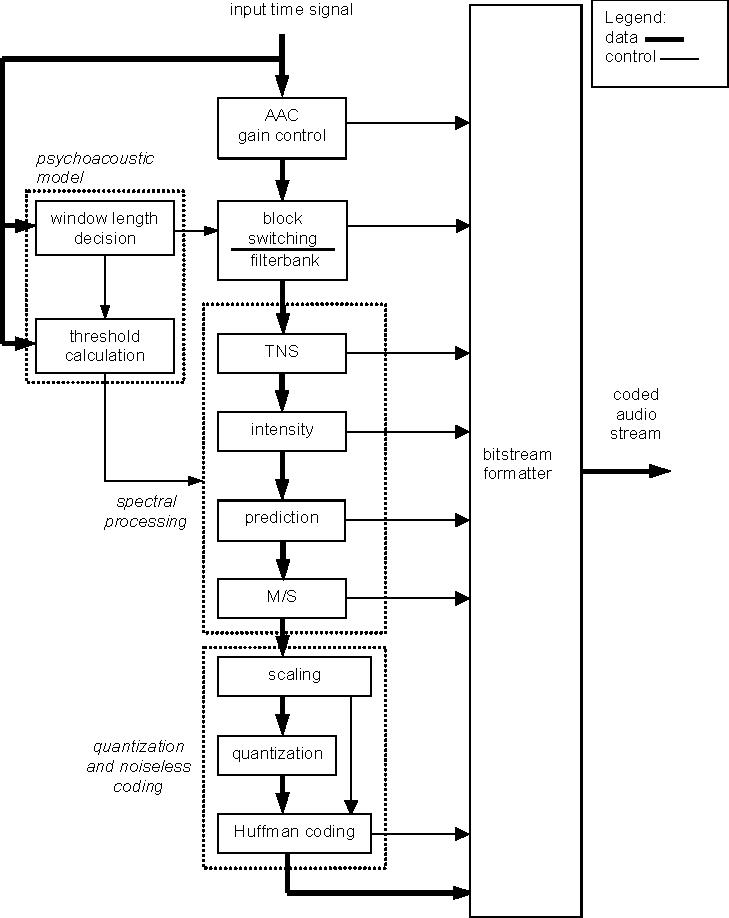
\includegraphics[width=.7\textwidth]{pic/aaclc.pdf}
    \caption{Blokové schéma AAC kodéru převzaté z normy \cite{iso:aac}}
    \label{pic:aaclc}
\end{figure}

Místo dělení signálu do několika desítek pásem pomocí filtrů v časové doméně, používá AAC LC profil modifikovanou\footnote{Modifikace transformace spočívá v úpravě transformačního jádra. Původně kosinový tvar se přibližuje obdélníkovému pulzu} kosinovou transformaci MDCT (\textit{Modified discrete cosine transform}) s proměnlivě dlouhými bloky. Ta je použita k převodu záznamu do 1024 frekvenčních subpásem, které jdou selektivněji kvantizovat výstupem psychoakustického modelu. Dále využívá vyrovnávací paměť pro zpětné adaptivní kódování. Pokud se v paměti kodéru nachází sekvence bitů, která je zrovna na vstupu, uloží se na výstup pouze její adresa. Jedná se o podobný přístup jako známé I, P a B snímky v pohyblivém obraze. V neposlední řadě používá AAC techniky jako jsou například TNS (\textit{Temporal Noise Shaping}), která \uv{posouvá} kvantizační šum nad slyšitelné pásmo, či JS (\textit{Joint Stereo}), které místo dvou plných kanálu ukládá jejich součet a jejich rozdíl, což je z hlediska entropie dat efektivnější.

Maximální bitová rychlost AAC závisí na vzorkovacím kmitočtu. Pro 44.1 kHz je to 264.6 kb/s, pro 48 kHz 288 kb/s. \cite{iso:aac}


\subsubsection{High Efficiency v1}

Vyšší kmitočty zabírají v tradičním kódování audiosignálů poměrně velkou část uložených dat. Ukazuje se ovšem, že z psychoakustického hlediska je exaktní reprodukce posledních jedné až dvou oktáv relativně nedůležitá. Při pouhém potlačení vyšších kmitočtů dolní propustí, jako to dělaly starší kodeky při nedostatečném datovém toku, ovšem označují posluchači vjem jako \uv{neúplný} či \uv{dutý} i přes zachování většiny relevantní informace. To společně s faktem, že z fyzikálního hlediska produkují hudební nástroje zvuky na ve spektru se periodicky opakujících kmitočtech, známých jako vyšší harmonické, vedlo k myšlence spektrální pásmové replikace (\textit{Spectral Band Replication}). Obrázek \ref{pic:sbr} naznačuje, jak takový proces probíhá na straně dekodéru. Pomocí transpozice je základní spektrum \uv{překopírováno} do pásma vyšších kmitočtů a poté je upravena spektrální obálka podle SBR dat vzniklých při kódování dat vstupního signálu. 

\begin{figure}[h]
    \centering
    \begin{subfigure}{.5\textwidth}
        \centering
        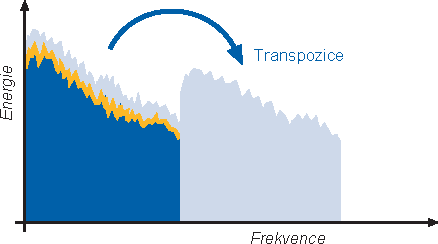
\includegraphics[width=1\linewidth]{pic/sbr1.pdf}
        \caption{Doplnění vyšších kmitočtů transpozicí.}
        \label{fig:sub1}
    \end{subfigure}%
    \begin{subfigure}{.5\textwidth}
        \centering
        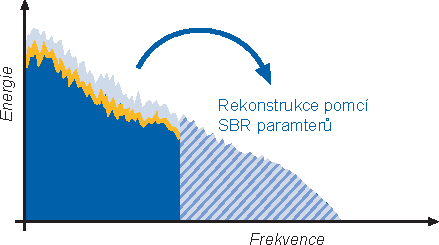
\includegraphics[width=1\linewidth]{pic/sbr2.pdf}
        \caption{Úprava energetické obálky.}
        \label{fig:sub2}
    \end{subfigure}
    \caption{Proces spektrální pásmové replikace.\cite{article:aac}} 
\label{pic:sbr}
\end{figure}
    
Při opětovném pohledu na obrázek \ref{pic:aac} vidíme, že kombinace AAC-LC v kombinaci se SBR tvoří profil známý pod jako \textit{High Efficiency AAC v1}. Tento princip obalování původního přístupu modernějšími technologiemi zajišťuje plnou zpětnou a částečnou dopřednou kompatibilitu.

Je nutno podotknout, že HE-AAC v1 není definován pro stejné bitové rychlosti jako jeho předchůdce. Při postupném snižování bitové rychlosti dostačuje kvalita \textit{Low Coplexity} profilu až do přibližně 128 kb/s. Při nižších datových tocích se již začíná být patrná přítomnost kompresních artefaktů. Snížení kvantizačního šumu lze dosáhnout pomocí zúžení pásma a právě tam nastupují výhody SBR.
    
\subsubsection{High Efficiency v2}
    
Profil známý jako HE-AAC v2 je dalším evolučním krokem v rodině kodeků AAC. Nad jeho předchozí verzi staví proces známý jako Parametrické Stereo PS (\textit{Parametric Stereo}). Podobně jako u SBR, které namísto původních dat využívá parametrického popisu obálkou, používá parametrické stereo signálovou podobnost. Tentokrát nikoli v kmitočtovém spektru ale v čase. Kodér ze vstupního signálu vezme levý a pravý kanál a smíchá je do jednoho \uv{monoaurálního} kanálu, jak naznačuje obrázek \ref{pic:ps}. Dále vypočítá z obou původních kanálů tři následující parametry:

    \begin{figure}[h]
        \centering
        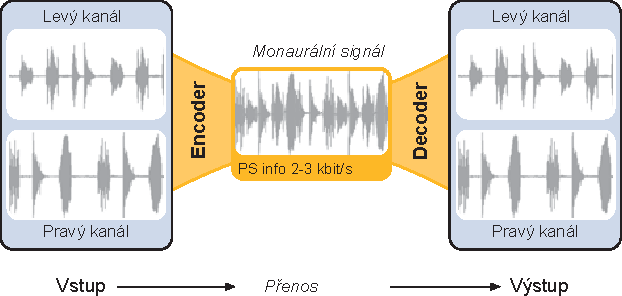
\includegraphics[width=.7\textwidth]{pic/parametricalStereo.pdf}
        \caption{Parametrické stereo \cite{article:aac}}
        \label{pic:ps}
    \end{figure}
    
    \begin{itemize}
        \item IID \textit{Inter-channel Intensity Difference} - Popisující rozdíl intenzity mezi jednotlivmi kanály. 
        \item ICC \textit{Inter-channel Cross-Correlation} - Vyjadřující míru koherence mezi jednotlivými kanály. Je vypočítán korelační funkcí.
        \item IPD \textit{Inter-channel Phase Difference} - Určující míru \uv{zpozdění} jednoho signálu vůči druhému.
    \end{itemize}
    
I tento profil se používá až při rychlostech, kdy již kvalita předchozích dvou profilů není dostatečná. 64 kb/s je maximální bitová rychlost při které lze parametrické stereo použít.
    
    \subsubsection{MPEG-D USAC}
    
Ať už jde o předčítání zpráv, diskuzní pořady či krátké vstupy moderátora mezi hudební reprodukcí, mluvené slovo je v rádiu velmi častým prvkem. Dlouhodobý vývoj přenosu řeči skrze digitální telefonní linku přineslo efektivní kódování mluveného slova zvané LPC (\textit{Linear Predictive Coding}). Vychází z poznatků o rezonanci zvukových vln v dutinách a dekompozici lidské řeči na elementy, které lze popsat databází. Na lidské hlasové ústrojí lze pohlížet jako na soustavu rezonančních trubic, ve kterých jsou zesíleny určité kmitočty, udávající barvu lidského hlasu. LPC analýza pomocí filtrů oddělí tyto kmitočty a vytvoří parametrický popis barvy hlasu. Ve zbytku signálu poté vyhledá řečové elementy a přiřadí jim prvky z databáze, kterou disponuje kodér i dekodér. Na přijímající straně je poté možno zrekonstruovat velmi věrně znějící repliku původního hlasu.

MPEG-D USAC (\textit{Unified Speech and Audio Coding}) vznikl myšlenkou spojit řečové AMR-WB+ (\textit{Extended Adaptive Multi-Rate – Wideband}) a hudební HE-AAC v2 kódování. Standard ISO/IEC 23003-3, známý pod označením MPEG-D, definuje nový přírůstek do rodiny AAC kodeků s názvem xHE-AAC (\textit{eXtended High Efficiency Advanced Audio Coding}) \cite{iso:usac},který cílí na bitové rychlosti 32 kb/s a nižší. Při pohledu na obrázek \ref{pic:aac} se může zdát, že xHE-AAC je jen dalším rozšířením, postaveným nad HE-AAC v2. Ve skutečnosti to tak ale není. USAC využívá stejných technologií jako jeho předchůdce, ale redefinuje většinu bloků aby bylo možné využít LPC analýzu. 

    \begin{figure}[h]
        \centering
        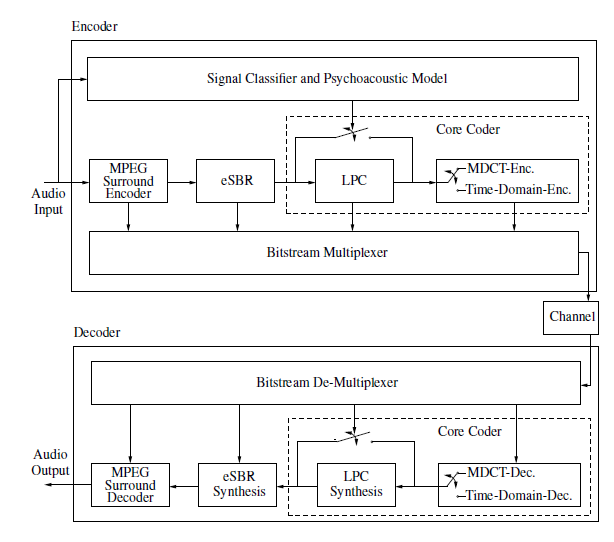
\includegraphics[width=.7\textwidth]{pic/usac.png}
        \caption{Kodér a dekodér xHE-AAC \cite{article:usac}}
        \label{pic:usac}
    \end{figure}
    
Na obrázku \ref{pic:usac} je naznačeno, jak kodek nakládá se vstupním signálem. Blok MPEG Surround produkuje parametrický popis stereofonního signálu a míchá kanály do jedné stopy. Ta je poté zpracována blokem eSBR (\textit{enhanced Spectral Band Replication}), který SBR použité v HE-AAC v2 doplňuje o efektivnější prediktivní vektorové kódování PVC (\textit{Predictive Vector Coding}). Jednokanálový nízkofrekvenční signál je poté po blocích zpracováván MDCT analýzou obdobnou té v Low Complexity profilu s volitelně doplněnou o LPC kodér. Volba přemostění řečového kódování lze vynutit natrvalo, či lze vypínat automaticky výstupem psychoakustického modelu rámec po rámci. Skokové přepínání mezi signálem kódovaným by mohlo produkovat kompresní artefakty. xHE-AAC proto definuje komplexní schéma přepínání mezi jednotlivými kódovacími metodami naznačené na obrázku \ref{pic:usac:switching}.

    \begin{figure}[h]
        \centering
        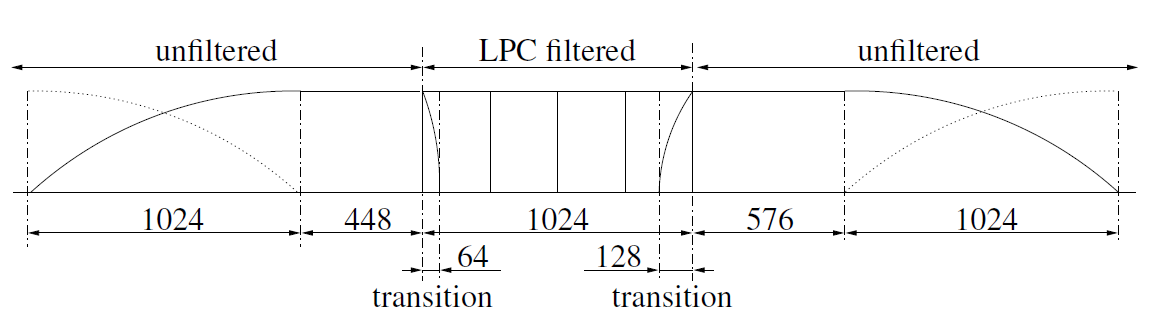
\includegraphics[width=.6\textwidth]{pic/switching.png}
        \caption{Schéma přepínání módů v USAC \cite{article:usac}}
        \label{pic:usac:switching}
    \end{figure}


\subsection{Opus}

Částečně mimo celou koncepci této práce stojí kodek jménem Opus. DAB ani DRM ho nemají ve svých definicích, i když na fóru \textit{HydrogenAudio} \cite{forum:hydro} jsou k nalezení zmínky tom, že s jistými úpravami lze Opus v DRM používat. To je nicméně velmi okrajová varianta a není důvodem proč je ve zdejším výčtu uveden. Skutečným důvodem pro jeho volbu byla jeho dostupnost. Je totiž jediným volně dostupným kodekem využívajícím sjednocené kódování řeči a hudby USAC. Srovnání s xHE-AAC by tedy mohlo být zajímavé.

Opus je standardizován pod záštitou IETF \textit{(Internet Engineering Task Force)} jako RFC6716 \cite{norm:opus}. Je relativně nový tj. jeho vývoj započal v roce 2007 a první verze spatřila světlo světa 11. Září 2012. V oficiálních materiálech autoři poskytují srovnání s velkým množstvím v současnosti používaných kodeků (obrázek \ref{pic:opus}), kde si vede velmi dobře.


\begin{figure}[h]
    \centering
    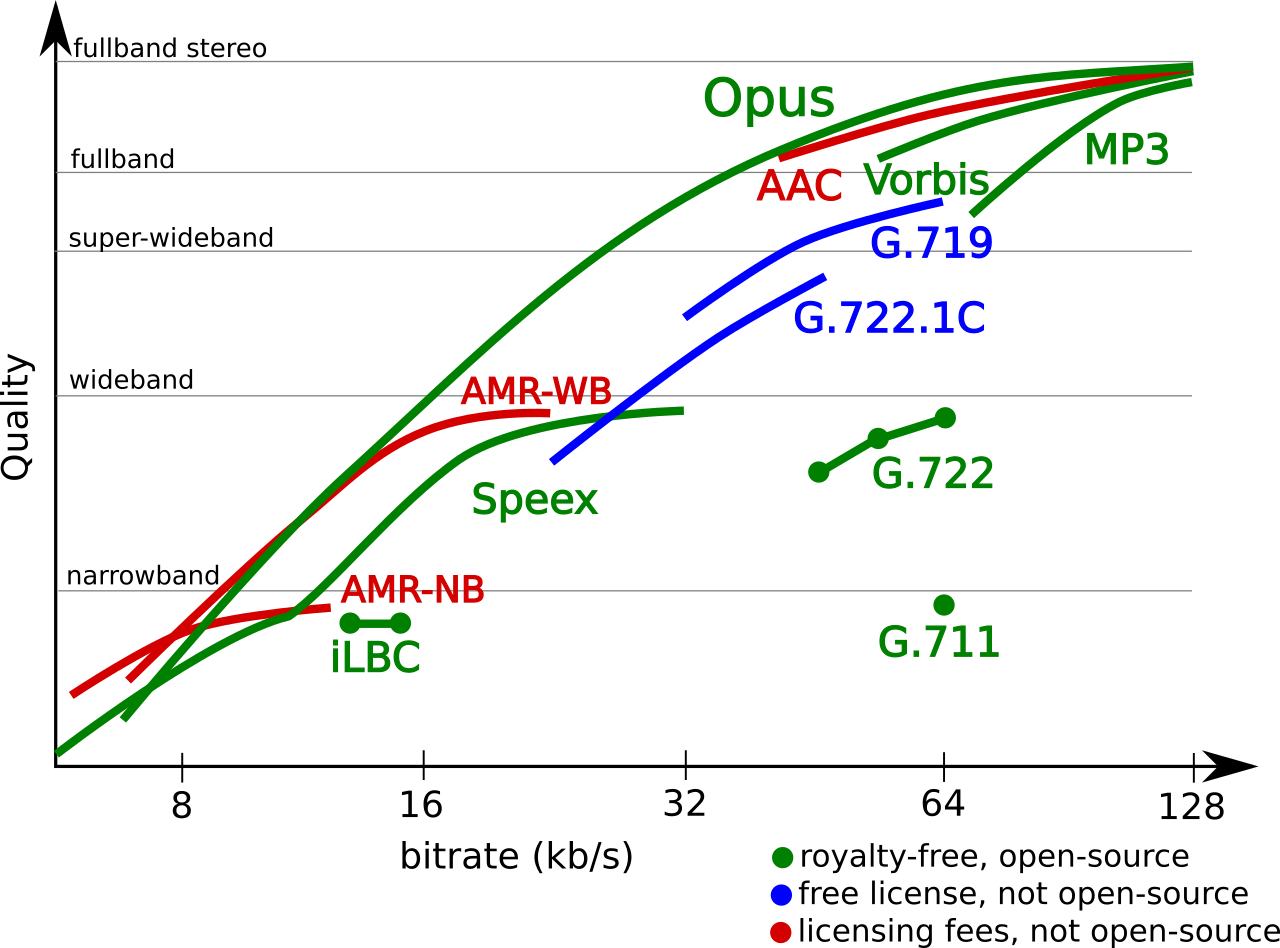
\includegraphics[width=.55\textwidth]{pic/opus.png}
    \caption{Srovnání kodeku Opus s ostatnímu kompresními metodami podle \cite{web:opus}}
    \label{pic:opus}
\end{figure}

Z technologického hlediska se velmi podobá xHE-AAC. Tam kde MPEG utilizuje řečové kódování AMR-WB+, využívá Opus kodek SILK vyvinutý společností Skype Technologies pro internetovou telefonii. Ke kódování zvuku používá CELT (\textit{Constrained Energy Lapped Transform}) otevřený kodek založený, stejně jako AAC, na MDCT analýze \cite{norm:opus}.